\documentclass[11pt]{amsart}


\usepackage[english]{babel}
\usepackage {amsmath} 
\usepackage{amssymb}
\usepackage{amsfonts}
\usepackage{amsthm}
\usepackage{graphicx}


\usepackage[colorlinks,linkcolor=blue, citecolor=blue,urlcolor=blue]{hyperref} % typesets URLS and clickable cross-references and links
%\usepackage{hyperref} % if you don't want colored links, just use the simpler command
\usepackage[backend=bibtex]{biblatex}

%% Environments for theorems, etc.. 
\theoremstyle{theorem} % set the style for the following theorems
\newtheorem{thm}{Theorem}[section] %\newtheorem{name}{display-text}[numbered-within]
\newtheorem{lem}[thm]{Lemma} %\newtheorem{name}[numbered-like]{display-text}
\newtheorem{cor}[thm]{Corollary}
\newtheorem{prop}[thm]{Proposition}
\newtheorem{alg}[thm]{Algorithm}
\theoremstyle{definition}                  % switch to a different style
\newtheorem{defn}[thm]{Definition}
\newtheorem{conj}[thm]{Conjecture}
\theoremstyle{example}                       % another style
\newtheorem{prob}[thm]{Problem}
\theoremstyle{remark}                       % another style
\newtheorem{exmp}[thm]{Example}  % (note:the "example" style is not really good for long examples-- typesets them in italics!)
\newtheorem{rem}[thm]{Remark}
\newtheorem{claim}[thm]{Claim}  
\renewcommand{\theclaim}{}
%% If you use numbered equations in a long document, it is preferred to number
% as (x.y), where x is section number, y is equation number

\numberwithin{equation}{section}


%% Common typesetting for common mathematical objects
\newcommand{\R}{\mathbb{R}}
\newcommand{\Q}{\mathbb{Q}}
\newcommand{\N}{\mathbb{N}}
\newcommand{\Z}{\mathbb{Z}}
\DeclareMathOperator{\rank}{rank}
\DeclareMathOperator{\dimension}{dim}

\addbibresource{wavelet.bib}

\title{Introduction to Wavelets in Image Processing}
\author{Jason Ngo}
\date{2019-01-21}

\begin{document}

\maketitle

\section{Introduction}
Since the start of the 20th century, we have seen rapid development in the theory and applications of wavelets. As a mathematical tool, wavelets can be used to extract information from different kinds of data such as audio signals and images.

This paper will explore what wavelets are, introduce readers to the first orthonormal wavelet basis: the Haar system, approximate functions using Haar wavelets, and discuss the applications of wavelets in image compression.

% exampes of wavelets (particularly the Haar wavelet), prove that wavelets form an orthonormal basis for $ L^2(\R) $ (and why we want a orthonormal basis in the first place), and its application to image compression (or edge detection of the Haar wavelets).

%The introduction for the smaller book in Wavelet chapter is pretty great. Get some ideas from them.
%
%This paper will aim to provide a general introduction to wavelets in the context of image processing.

%
%We can explore the case study of FBI Fingerprint compression (pull stories from the two books).
%
%Maybe I can include a short description of Fourier series// Comparisons between Wavelet and Fourier. and show why wavelets are better.
%
%Compression applications: when compressing images, we want to discard the least significant details, keeping the original picture largely intact. Wavelets are superior to Fourier series in this sense because we can isolate and decompose a signal (a picture is just a bunch of pixels and can be represented as signals) into low frequency part and high frequency part. If we remove the high frequency, we get a smoother representation of the figure.
%
%Haar basis is very good for edge detection. Maybe talk about this.
%
%``Along this vein, the book by Strang and Nguyen describes a widely used application of wavelets, fingerprint compression, in which edge detection figures prominently." (Standford book)
%
%\section{Research Hypothesis/Question}
%
%Davidson and Donsig does give a terse proof why the Haar wavelets system forms an orthonormal basis for $ L^2(\R) $. My job is to take ownership of the proof by rewriting it, come up with examples/illustrations, and a discussion of why we want the Haar Wavelets system to form an orthonormal basis in the context of edge detection.
%
%After proving these properties of Haar Wavelet, I can go into the application in edge detection (or whatever application that I decided on). This part will likely use some Linear Algebra and visualization.
%
%So the bulk of the mathematical reasoning will be in the proof that Haar system is orthonormal. I'm not sure if this is sufficient or not. But I can read more about the application of the Haar system, and see what properties are needed for that application. I can then proceed to prove those properties.

\section{Definitions}
\begin{defn} \label{def:l2}
	\emph{$ L^2(\R) $ space} is the set of all functions $ f: \R \to \R $ such that the integral of $ f^2 $ over the whole real line is finite, taken with the norm
	\[ \|f\|_2^2 = \int_{-\infty}^{\infty} |f(x)|^2 dx. \]
	
\end{defn}

\begin{defn} \label{def: wavelet}
	A \emph{wavelet} is a function $ \varPsi \in L^2(\R) $ such that the set
	\[ \{ \varPsi_{j,k}(x) = 2^{j/2} \varPsi (2^j x-k): j,k \in \Z  \} \]
	forms an orthonormal basis for $ L^2(\R) $. Sometimes $ \varPsi $ is called the \emph{mother wavelet}.
\end{defn}

	Observe that all $ \varPsi_{j,k} $ are generated by shifting and scaling\footnote{The dilations here are taken to be powers of 2.} the wavelet $ \varPsi $ and that each $ \varPsi_{j,k} $ is normalized so that $ \| \varPsi_{j,k}\|_2 = \|\varPsi\|_2 = 1 $ for all $ j,k \in \Z $.
	
	Now, let us explore one particular type of wavelet that has many applications in noise filtering and image processing: \emph{The Haar Wavelet}. To get started, let $ \chi_{[a,b)} $ denote the characteristic function\footnote{The function defined to be identically one on $ [a,b) $, and is zero elsewhere.} of the interval $ [a,b) $.
	
\begin{defn}
	The \emph{Haar wavelet} is the function $ \varPsi = \chi_{[0,0.5)} - \chi_{[0.5,1)} $. The \emph{Haar wavelet basis is the family $ \{ \varPsi_{j,k}:j,k \in \Z \} $}.
\end{defn}
See Figure \ref{fig:haarsystem} for some elements of the Haar wavelet basis, obtained by translating and/or stretching the Haar wavelet. 

\begin{figure}[h]
	\centering
	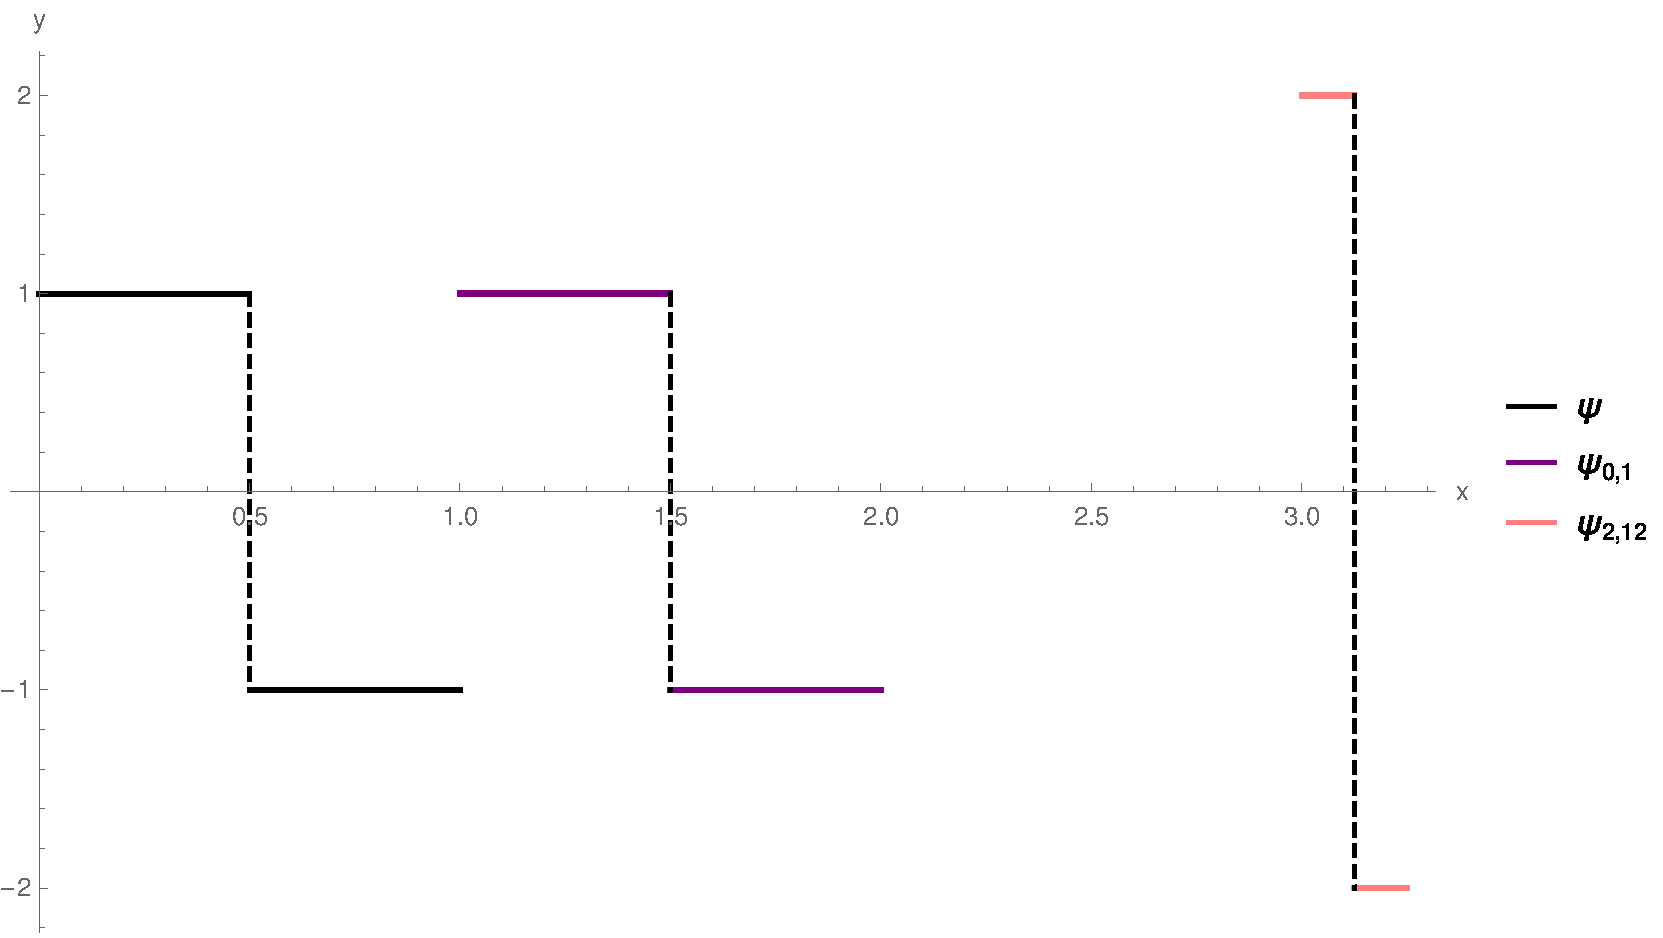
\includegraphics[width=0.7\linewidth]{img/haar_system}
	\caption[Elements of the Haar system]{Elements of the Haar system: $ \varPsi, \varPsi_{0,1} $ and $ \varPsi_{2,12} $}
	\label{fig:haarsystem}
\end{figure}

Now, our task is to prove that the Haar wavelet is in fact a wavelet, i.e. the Haar wavelet basis is an orthonormal basis for $ L^2(\R) $.

\section{Haar wavelet basis}
\begin{lem}
	The Haar system is an orthonormal set in $ L^2(\R) $.
\end{lem}

\begin{defn}
	Set $ \varphi = \chi_{[0,1)} $. Define the sequence of partial sums to be:
	\[ H_n f(x) = \langle f, \varphi \rangle \varphi(x) + \sum_{j=0}^{n-1} \sum_{k=0}^{2^j-1} \langle f, \varPsi_{j,k} \rangle \varPsi_{j,k} (x). \]
\end{defn}

\begin{lem}
	Let $ f \in L^2(0,1) $. Then $ H_nf $ converges to $ f $ in the $ L^2 $ norm. Consequently, the Haar system is an orthonormal basis for $ L^2(0,1) $. Moreover, if $ f $ is continuous on $ [0,1] $, then $ H_nf $ converges uniformly to $ f $.
\end{lem}

\begin{thm}
	The Haar wavelet basis spans all of $ L^(\R) $.
\end{thm}

\section{Approximations using Haar wavelets}
\begin{thm}
	If $ f \in C_0(\R) $, then the series $ \sum_{j,k \in \Z} \langle f, \varPsi_{j,k} \rangle \varPsi_{j,k} $ converges to $ f $ uniformly on $ \R $.
\end{thm}

\begin{exmp}
	Consider $ f(x) = e^{-x} \sin 2\pi x $ for $ x \in (0,1) $.
	
	See Figure \ref{fig:approximations} 
\end{exmp}

\begin{figure}[h]
	\centering
	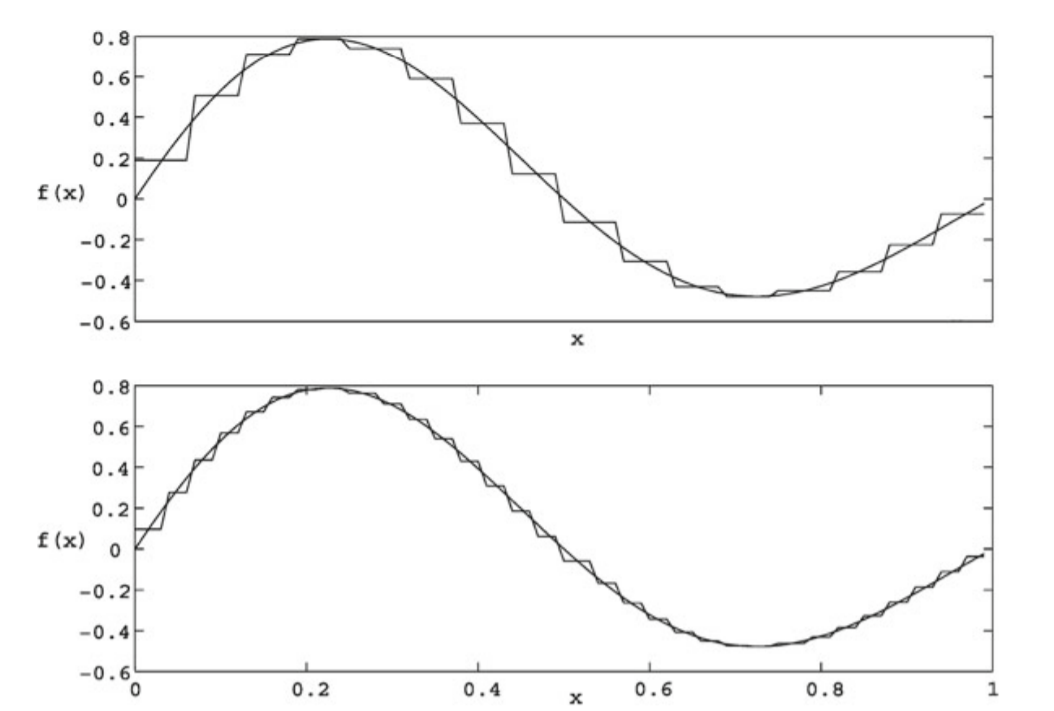
\includegraphics[width=0.7\linewidth]{img/approximations}
	\caption{Approximations of $ f(x) = e^{-x} \sin{2\pi x} $ using Haar wavelets}
	\label{fig:approximations}
\end{figure}


\section{Application to Image Processing}
 When compressing images, we want to discard the least significant details, keeping the original picture largely intact. Fortunately, wavelets can isolate and decompose a signal into low frequency part and high frequency part.
 Briefly discuss FBI Fingerprint Image Compression if there is space:
 \begin{quote}
 	 Wavelet compression methods do not require dividing the image into smaller blocks because the desired localization properties are naturally built into the wavelet system.\cite{Frazier_1999}
 \end{quote}
 
\section{Annotated Bibliography}
\begin{enumerate}
	\item \fullcite{davidson_real_2002}
	
	\smallskip
	This textbook is my primary source for proofs of orthonormal basis. Though terse, the book introduces the lemmas and proofs in a logical way, starting with proving the Haar system is orthonormal and then expand it to the basis for $L^2(\R)$.
		
	\item \fullcite{Frazier_1999}
	
	\smallskip
	This textbook is very introductory, including a lot of examples and step-by-step proof for the properties of wavelets. Furthermore, it also has a nice description of the FBI Fingerprint Compression application using Haar Wavelets Analysis.	
	
	\item \fullcite{Gomes_Velho_2015}
	
	\smallskip
	Although this textbook is not very proof-heavy, it brings up a lot of cool wavelet examples that pertain to image compression, one of which being the Blur Derivative that I can talk about in my first draft.
\end{enumerate}

\end{document}

